Although the concepts and definitions of combinatorial game theory have impact in general mathematics, it is a relatively new field of study that has many open problems and not so many resources or implementations available. The purpose of this section is to bring examples, pieces of code and discuss a particular software that implements most of the theory discussed up to this point. The code fragments featured in the text follow C++ syntax, with the intent of being as simple as possible.

The examples and code fragments also serve the purpose of showing possible readers that the theory is actually quite simple, not requiring great mathematical skills, and that applying it is also not difficult. With them, some concepts presented will become clearer and a few facts enunciated will be shown. A second part of this section will introduce a few new games so that the reader might find other interesting games to play. In this second part, the reader will also see that it is not hard to make up fun games on the spot. This section can work as a midpoint between presenting the concepts and a shift in focus to handle the problem of temperature bounding, and may serve to verify if the concepts are clear.

\subsection*{The Numbers}

A very important and recurrent theme in the early parts of the text is the correspondence between games and surreal numbers. It is correct to say that all real numbers are also games, but it may not be clear how to make a particular real number. For example, the reader may not be able to make a game with value equals to $\pi$. In fact, the reader may not know what numbers are easy or hard to do. For now, the first two rules of the simplicity principle should be clear enough.

\begin{lstlisting}[language=C++]
using std::max, std::floor, std::vector, std::unique_ptr;

// Initial class structure
class SurrealNumber {
  public:
	float toFloat ();
	...
  private:
  	vector<unique_ptr<SurrealNumber>> left;
  	vector<unique_ptr<SurrealNumber>> right;
  	...
};

float SurrealNumber::toFloat () {
	float ret;
	if (left.empty())
		if (right.empty())
			ret = 0.0f;
		else
			ret = min(floor(${-}$1 + minRight()->toFloat()), 0.0f);
	else if (right.empty())
		ret = max(floor(1 + maxLeft()->toFloat()), 0.0f);
	// other cases
	...
	return ret;
}
\end{lstlisting}

While easy and hard is relative, every number that is a dyadic rational, a number that is of the form $\frac{a}{2^b}, a\in\mathbb{Z}, b \in \mathbb{N}$ is easy to form. A good method to make the representation of $z = \frac{a}{2^b}, z \ge 0$ in \gam{x}{y} is:\\
\begin{adjustwidth}{2cm}{}
	1) Calculate $d\in \mathbb{Z}\;|\;0 \leq z-d < 1$.\\
	2) If $z=d$ then $x = z-1,y=z+1$, stop.\\ 
	3) Binary search for any $w = z-d \in(0,1)$\\
	4) $x$ is $d$ added to the oldest number to the left.\\
	6) $y$ is $d$ added to the oldest number to the right.
\end{adjustwidth} \vspace{0.5cm}

For example, $\frac{89}{16} = 5 + \frac{9}{16} = \gam{5 + \frac{1}{2}}{5+\frac{5}{8}}$, because the binary search for $\frac{9}{16} = \frac{89-80}{16}$ follows the path $\frac{1}{2}\xrightarrow[]{R} \frac{3}{4}\xrightarrow[]{L}\frac{5}{8}\xrightarrow[]{L}\frac{9}{16}$. In RB-Hackenbush, building $\frac{89}{16}$ is now easy. Take a pile with five blue edges and add it to a blue-red-blue-blue pile. The red-blue-blue pile on top of that derives from the right-left-left path on the binary search for $\frac{9}{16}$, with a right turn corresponding to a red edge and vice-versa. Therefore, it is possible to complement the featured snippet, repeating the idea, but with the objective of finding $z = \frac{a}{2^b}$ given \gam{X}{Y}.

\begin{lstlisting}[language=C++]
	//other cases
	else {
		float maxL = maxLeft();
		float minR = minRight();
		if (maxL < 0 && 0 < minR)
			return 0.0f;
		float d = floor(maxL);
		maxL -= d; minR -= d;
  		float fact = 1.0f;
		while (fact > 1.0f/4096.0f)
			if (x < fact)
				if (y > fact)
					break;
				else
					fact *= 0.5f;
			else
				fact *= 1.5f;
		ret = d + fact;
	}
\end{lstlisting}

All the remaining numbers are hard in the sense that they require an infinite number of steps to define. A simple code like the one above will not handle that. That is because $\frac{2}{3}$ and $\pi$ are both generated in the $\aleph$th day (section 3), like any other non-dyadic fraction. However, these are not equally hard. Because $\frac{2}{3}$ is a periodic number when using binary representation, its path in the numbers tree is well-defined.

It is true that both $\frac{2}{3}$ and $\pi$ are given by something equivalent to the following: $n = \gam{x \in S_*:x < n}{y \in S_*:y>n}$, where $S_*$ is the set of numbers generated until day $\aleph$. However, $\frac{2}{3}=0.\overline{10}_2$ can also be defined through the infinite right-left-right-left... path in the binary tree, because a 1 in the binary representation is a step do the right in the tree and vice-versa. One way to think of this fact is that, when doing a binary search for $x$ between the dyadics in (0,1), the starting question is $x > 1/2$. The 1 indicates a yes, so the following question is $x > 3/4$, and so on. Since numbers smaller than $x$ go on the left set and vice-versa, $\frac{2}{3} = \gam{1/2, 5/8, \ldots}{3/4,11/16,\ldots}$, showing that the numbers visited in the binary search alternate in the left and right sets. Repeating decimals, in RB-Hackenbush, are extremely easy to spot because they are always a sequence of reds and blues followed by a finite pattern repeated infinitely.

Other than some real numbers being hard to draw, drawing non-reals is also not trivial. It was shown that there are infinitely many numbers between any two real numbers, in section 3. This might seem hard to understand or accept initially, because the reals form the complete ordered field. However, at least based on Conway surreal numbers, the fact that it is possible to build a game in which the advantage a player has is strictly between two real numbers gives some light to the fact. To do that, simply add an infinitesimal to a real number. For example:

\begin{center}
	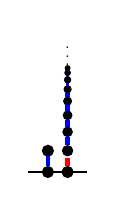
\begin{tikzpicture}
		\begin{scope} [every node/.style={scale=0.3, style=circle, draw, fill=black}]
			\node [scale=1.4] (1) at (0, -1.80){};
			\node [scale=1.3] (2) at (0, -1.26){};
			\node [scale=1.2] (3) at (0, -0.78){};
			\node [scale=1.1] (4) at (0, -0.36){};
			\node [scale=1]   (5) at (0, 0)      {};
			\node [scale=0.9] (6) at (0, 0.3)  {};
			\node [scale=0.8] (7) at (0, 0.54) {};
			\node [scale=0.7] (8) at (0, 0.72) {};
			\node [scale=0.6] (9) at (0, 0.84) {};
			\node [scale=1.4] (10) at (-0.5, -1.80) {};
			\node [scale=1.4] (11) at (-0.5, -1.26) {};
			\node [scale=0.2, fill=white, draw=none] at (0, 1.1) {$\vdots$};
		\end{scope}
		\draw (-1,-1.80) -- (0.5, -1.80);
		\draw[red, densely dashed, ultra thick] (1)--(2);
		\draw[blue, ultra thick] (2)--(3);
		\draw[blue, ultra thick] (3)--(4);
		\draw[blue, ultra thick] (4)--(5);
		\draw[blue, ultra thick] (5)--(6);
		\draw[blue, thick] (6)--(7);
		\draw[blue, thick] (7)--(8);
		\draw[blue] (8)--(9);
		\draw[blue, ultra thick] (10)--(11);
		\node[scale=1.5] at (0, 1.3) {\scriptsize$\vdots$};
	\end{tikzpicture},
\end{center}

has value $1-\epsilon$, a number smaller than 1, but larger than any $x \in \mathbb{R}, x < 1$. Although the non-reals might be new, the effort of writing hard reals and non-reals as RB-Hackenbush is very similar.

RB-Hackenbush is an extremely good example to understand numbers, as finding dyadics and repeating decimals are very easy. However, not all games are like this. It was shown that
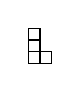
\begin{tikzpicture}
	\draw[] (0.3,-0.3) rectangle ++(0.3,0.3);
	\draw[] (0,-0.3) rectangle ++(0.3,0.3);
	\draw[] (0,0) rectangle ++(0.3,0.3);
	\draw[] (0,0.3) rectangle ++(0.3,0.3);
\end{tikzpicture} = $\frac{1}{2}$, but how would one build an instance of $\frac{1}{4}$, or $\frac{1}{2^n}$, for $n\in\mathbb{N}$? It turns out that it is not trivial at all.

In fact, only in 1996 a partial solution was given. One of the results of the paper ``New Values in Domineering" \cite{10} was the existence of arbitrarily small values of domineering games. Before that, it was unknown whether or not they existed. It was only in 2015 \cite{11} that a method to create all dyadic rationals was introduced. Following the strategy presented in 1996, the so-called Yonghoan Kim's snakes were created, named after the author. The snake's representation is found below, copied from Richard K. Guy's list of unresolved problems in \textit{Games of no Chance} \cite{GONC}:

\vspace{1cm}\hspace{-2cm}
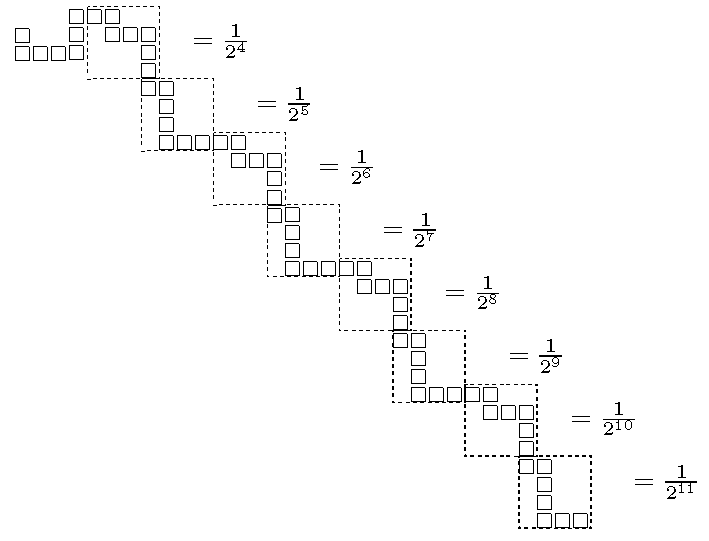
\includegraphics[scale=0.9]{../images/kims_snakes.png}

In this method of finding dyadics, there is a initial structure, that is not marked by a dashed rectangle. To this structure, additional ones are appended. As shown, each additional structure alternated between two others. Of course that the resulting game is not the only game with the given values.

In fact, there are special games with the same value as the snakes. The 2015 paper is based on these special games. This special games are based on concatenating and imploding bridges in domineering games. Bridges are cells that do not change the value of a game. For example, 
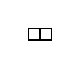
\begin{tikzpicture}
	\draw[] (0.3,0) rectangle ++(0.3,0.3);
	\draw[] (0,0) rectangle ++(0.3,0.3);

\end{tikzpicture}
and
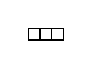
\begin{tikzpicture}
	\draw[] (0.9,0) rectangle ++(0.3,0.3);
	\draw[] (1.2,0) rectangle ++(0.3,0.3);
	\draw[] (1.5,0) rectangle ++(0.3,0.3);
\end{tikzpicture}
have the same value, so one of the extremities is a bridge. The strategy is built upon two theorems that are beautiful because they are powerful yet very simple.

The \textit{Bridge Splitting Theorem for Domineering} was introduced by Conway's. It reads:
If the value of \Gm{}\begin{tikzpicture}\draw[] (0.1,0) rectangle ++(0.3,0.3);\end{tikzpicture} is the same as \Gm{}, then the value of \Gm{}\begin{tikzpicture}\draw[] (0.1,0) rectangle ++(0.3,0.3);\end{tikzpicture}\Hm{} is the sum of the values of \Gm{} and \begin{tikzpicture}\draw[] (0.1,0) rectangle ++(0.3,0.3);\end{tikzpicture}\Hm{}, given \Gm{} and \Hm{} do not intersect. The proof is:

$$
\Gm{}\begin{tikzpicture}\draw[] (0.1,0) rectangle ++(0.3,0.3);\end{tikzpicture}\Hm{} \leq \Gm{} + \begin{tikzpicture}\draw[] (0.1,0) rectangle ++(0.3,0.3);\end{tikzpicture}\Hm{} = 
\Gm{}\begin{tikzpicture}\draw[] (0.1,0) rectangle ++(0.3,0.3);\end{tikzpicture} + \begin{tikzpicture}\draw[] (0.1,0) rectangle ++(0.3,0.3);\end{tikzpicture}\Hm{} \leq
\Gm{}\begin{tikzpicture}\draw[] (0.1,0) rectangle ++(0.3,0.3);\end{tikzpicture}\Hm{}
$$

The first inequality since splitting a horizontal always favors Right, and, the second inequality is true because merging horizontal squares also do always favor Left. The second important theorem was created by the authors.

\textit{Bridge Destroying Theorem for Domineering}

If the value of \Gm{}\begin{tikzpicture}\draw[] (0,0) rectangle ++(0.3,0.3);\end{tikzpicture}, 
\begin{tikzpicture}\draw[] (0,0) rectangle ++(0.3,0.3);\node at (0.15, 0.5) {$H$};\end{tikzpicture}, 
\begin{tikzpicture}\draw[] (0.1,0) rectangle ++(0.3,0.3);\end{tikzpicture}$I$
 and
\begin{tikzpicture}[baseline={(current bounding box.center)}]\draw[] (0,0) rectangle ++(0.3,0.3);\node at (0.15,-0.2){$J$};\end{tikzpicture}
 are the same of the values of $G$, $H$, $I$, $J$, then the value of
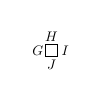
\begin{tikzpicture}[baseline={(current bounding box.center)}]
	\draw[] (0,0) rectangle ++(0.3,0.3);
	\node at (-0.2, 0.15) {$G$};
	\node at (0.15, 0.5) {$H$};
	\node at (0.5, 0.15) {$I$};
	\node at (0.15,-0.2){$J$};
\end{tikzpicture}
is the same as the sum of $G, H, I$ and $J$, provided that neither of the games have common edges. The proof is also simple:

$$
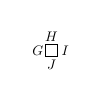
\begin{tikzpicture}[baseline={(current bounding box.center)}]
	\draw[] (0,0) rectangle ++(0.3,0.3);
	\node at (-0.2, 0.15) {$G$};
	\node at (0.15, 0.5) {$H$};
	\node at (0.5, 0.15) {$I$};
	\node at (0.15,-0.2){$J$};
\end{tikzpicture} \leq
G + \begin{tikzpicture}[baseline={(current bounding box.center)}]
	\draw[] (0,0) rectangle ++(0.3,0.3);
	\node at (0.15, 0.5) {$H$};
	\node at (0.5, 0.15) {$I$};
	\node at (0.15,-0.2){$J$};
\end{tikzpicture} \leq
G + I + \begin{tikzpicture}[baseline={(current bounding box.center)}]
	\draw[] (0,0) rectangle ++(0.3,0.3);
	\node at (0.15, 0.5) {$H$};
	\node at (0.15,-0.2){$J$};
\end{tikzpicture} =
G + H + I + J =
$$
$$
= H + J + \begin{tikzpicture}[baseline={(current bounding box.center)}]
	\draw[] (0,0) rectangle ++(0.3,0.3);
	\node at (-0.2, 0.15) {$G$};
	\node at (0.5, 0.15) {$I$};
\end{tikzpicture} \leq
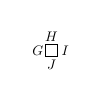
\begin{tikzpicture}[baseline={(current bounding box.center)}]
	\draw[] (0,0) rectangle ++(0.3,0.3);
	\node at (-0.2, 0.15) {$G$};
	\node at (0.15, 0.5) {$H$};
	\node at (0.5, 0.15) {$I$};
	\node at (0.15,-0.2){$J$};
\end{tikzpicture}
$$

The first two inequalities are true because they both split a horizontal line, favoring right. The two equalities are true because they are applications of the \textit{Bridge Splitting Theorem for Domineering}. The last inequality is true because is a linking of a vertical line, which can only favor Left.

An example of applying this is figuring out that 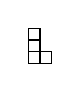
\begin{tikzpicture}
	\draw[] (0.3,-0.3) rectangle ++(0.3,0.3);
	\draw[] (0,-0.3) rectangle ++(0.3,0.3);
	\draw[] (0,0) rectangle ++(0.3,0.3);
	\draw[] (0,0.3) rectangle ++(0.3,0.3);
\end{tikzpicture} =
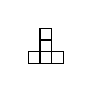
\begin{tikzpicture}
	\draw[] (0.3,-0.3) rectangle ++(0.3,0.3);
	\draw[] (0,-0.3) rectangle ++(0.3,0.3);
	\draw[] (-0.3,-0.3) rectangle ++(0.3,0.3);
	\draw[] (0,0) rectangle ++(0.3,0.3);
	\draw[] (0,0.3) rectangle ++(0.3,0.3);
\end{tikzpicture} = $\frac{1}{2}$, therefore it is true that 
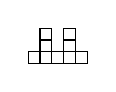
\begin{tikzpicture}
	\draw[] (0.3,-0.3) rectangle ++(0.3,0.3);
	\draw[] (0,-0.3) rectangle ++(0.3,0.3);
	\draw[] (-0.3,-0.3) rectangle ++(0.3,0.3);
	\draw[] (0.6,-0.3) rectangle ++(0.3,0.3);
	\draw[] (0.9,-0.3) rectangle ++(0.3,0.3);
	\draw[] (0,0) rectangle ++(0.3,0.3);
	\draw[] (0,0.3) rectangle ++(0.3,0.3);
	\draw[] (0.6,0) rectangle ++(0.3,0.3);
	\draw[] (0.6,0.3) rectangle ++(0.3,0.3);
\end{tikzpicture} $=1$. Another, much more beautiful example is given on 2015 paper:

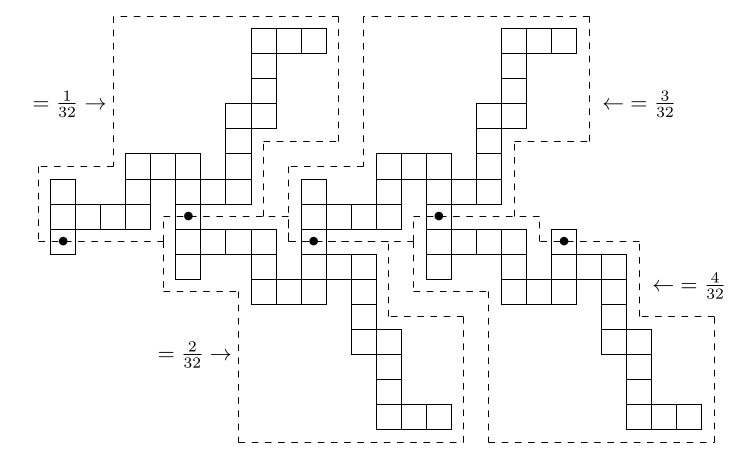
\includegraphics[scale=0.5]{../images/dyadic_domineering.png}

By combining the two theorems with Kim's snakes, it would be possible to create any dyadic in a single connected component, if not for two problems. The first is the problem of creating a bridge. However, that is a non-problem because the theorems mentioned above are enough to provide explosive squares. An explosive square that is always there is a square below the two vertical squares to the left of the base configuration of Kim's snakes. Since the value of the snake is equal to the values of the sum of the bridged components, the base component may be interchanged with the one with an explosive square and the values of the snake would remain the same.

The second problems is that of making sure ever component will not share an edge with the others. The solution of this second problem is fond on the aforementioned paper. The domineering discussion above serves to show how some games are good to analyse and create examples with, while other not so much. Another examples of that was the game "Extended Simpler Cashing Cheques (ESCC)". 

\subsection*{The non-numbers}

When the topic changed from numbers to non-numbers, an example of ambient temperature, and how it affected play, was required. In order to keep the results to the boundaries of the literature, an instance of this game was showed. This instance was made by reverse engineering the example of the same topic found on \textit{Winning Ways} \cite{WW} in this convenient game. Normally, it is extremely hard to generate a configuration with any temperature value, but ESCC allows it, and this is why its creation in this text was important.

ESCC allows an easy conversion from a \gam{X}{Y} to a configuration, mainly because any switch is trivial to write down. The thermograph found in domineering is copied below:

\vspace{0.5cm}\hspace{-3cm}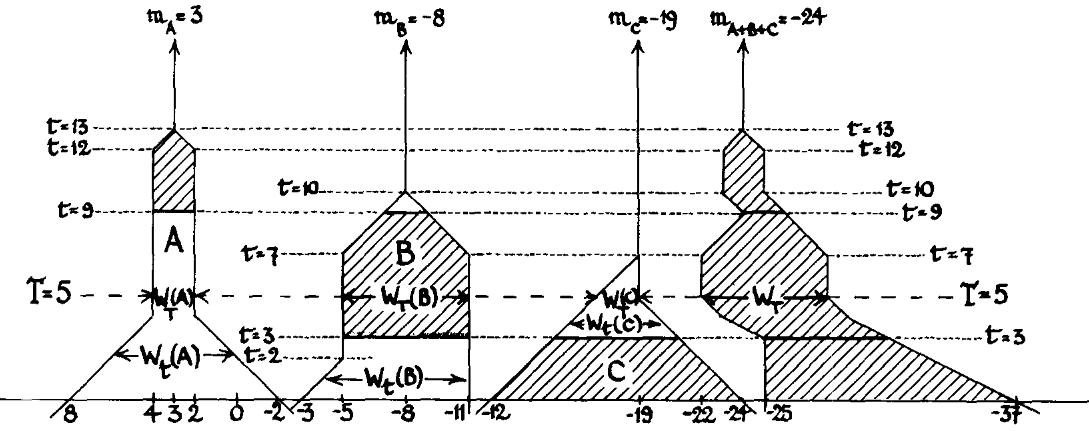
\includegraphics[scale=0.5]{../images/cpd_therm_ww.png}
\vspace{0.5cm}

To verify that the resulting compounded thermograph of the example featured in the previous section is indeed the one found above, it is possible to use Aaron Siegel's CGSuite. CGSuite is an implementation of almost all of the methods found in Combinatorial Game Theory. This text will not go in detail on the programming language used in the engine, but will bring to light some information.

Between other practical and interesting features, it is possible to create any games and calculate and plot their thermographs. For example:

\begin{center}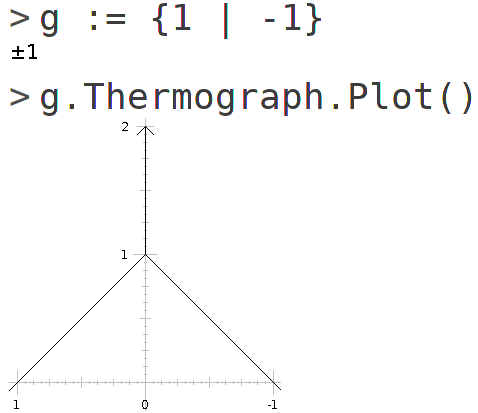
\includegraphics[scale=0.3]{../images/cgsex1.png}\end{center}

The game from last section could, then, be converted to the following:

\begingroup
\tikzset{every picture/.style={scale=0.5}, every node/.style={scale=0.5}}%
\begin{figure}[H]
\begin{center}
	\scalebox{0.9}{
	\begin{tikzpicture}
		\node[draw] (title) at (3,1.5) {\textbf{Extended Simpler Cashing Cheques}};
		\begin{scope} []
			\draw[fill=yellow] (-1,-1) rectangle ++(8,1.9);
			\draw[fill=yellow] (0,-3) rectangle ++(6,1.9);
			\draw[fill=yellow] (0,-5) rectangle ++(6,1.9);
			\node[] at (-2,0) {\Large A};
			\node[] at (-1,-2) {\Large B};
			\node[] at (-1,-4) {\Large C};
			\node[circle, draw, fill=purple2] at (0,0) {7 $|$ {-}9};
			\node[circle, draw, fill=purple2] at (2,0) {28 $|$ {-}4};
			\draw[thick] (3,-0.75) -- (3,0.75);
			\node[circle, draw, fill=purple2] at (4,0) {{-}3 $|$ 1};
			\node[circle, draw, fill=purple2] at (6,0) {2 $|$ 22};
			\node[circle, draw, fill=purple2] at (1,-2) {{-}4 $|$ 2};
			\node[circle, draw, fill=purple2] at (3,-2) {9 $|$ 5};
			\draw[thick] (4,-2.75) -- (4,-1.25);
			\node[circle, draw, fill=purple2, scale=0.9] at (5,-2) {{-}11 $|$ {25}};
			\node[circle, draw, fill=purple2, scale=0.95] at (1,-4) {{-13} $|$ 11};
			\draw[thick] (2,-4.75) -- (2,-3.25);
			\node[circle, draw, fill=purple2, scale=0.94] at (3,-4) {{-}25 $|$ 23};
			\node[circle, draw, fill=purple2] at (5,-4) {{-}19 $|$ 35};
		\end{scope}
	\end{tikzpicture}
}
\end{center}
\caption{Sum of hot components without dominated moves}
\end{figure}
\endgroup
\begin{center}
	$\Downarrow$
\end{center}
\begin{center}
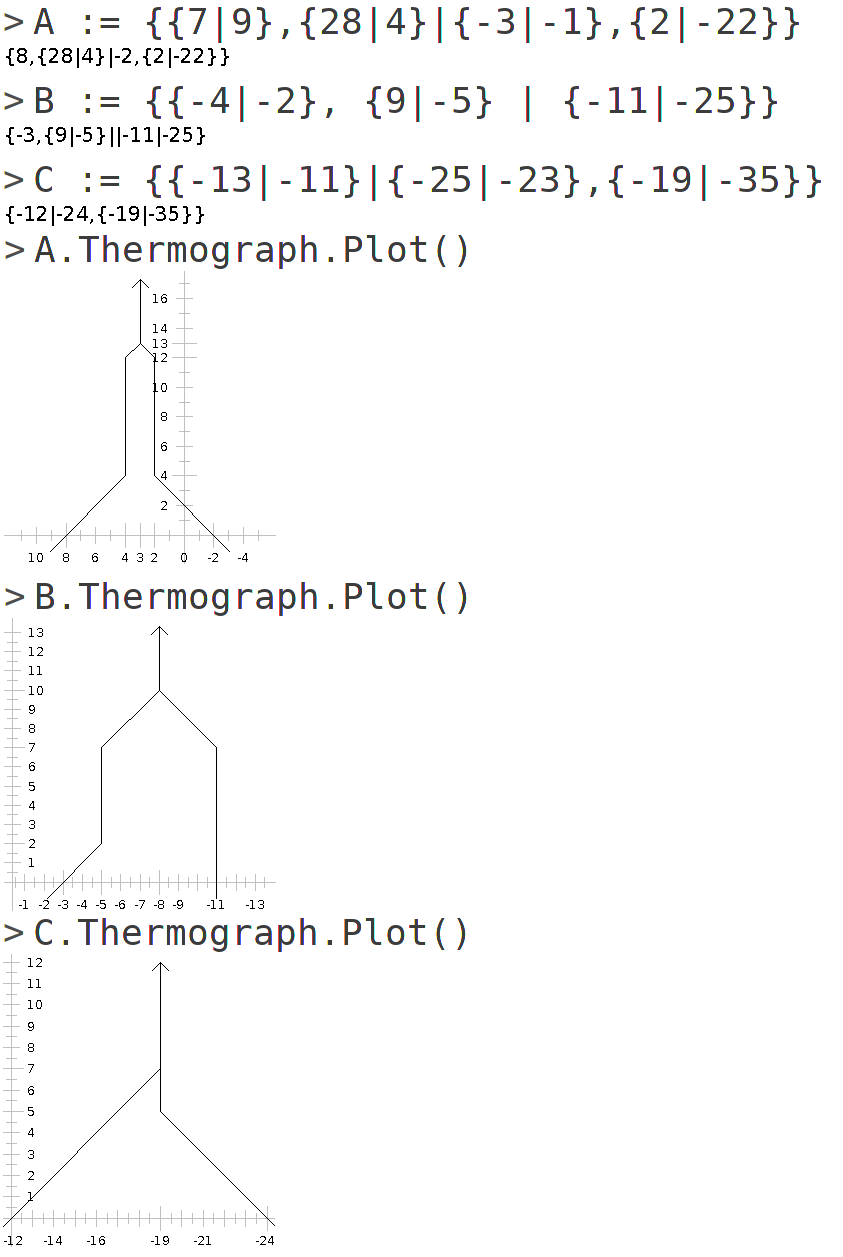
\includegraphics[scale=0.3]{../images/resulting_thermographs.png}
\end{center}

Therefore the game from last section is indeed the same as the one featured in the book. The steps taken to reverse engineer the games whose thermographs were the ones indicated in the book, might be of useful to speed up the process of calculating and exercising the process of building thermographs by head. This process uses a theorem not yet mentioned.

This theorem is about the structure of thermographs. It states that every line in a thermograph has slope equals to ${-}1$, $0$ or $1$ and masts have slope 0. Using the notation created by Aaron \cite{CGT}, let $G$ be a game and $\lambda_t(G), \rho_t(G)$ its thermograph's left and right trajectories, respectively. It means that:

\begin{align*}
\overset{\sim}{\lambda}_t(G) =&\; \underset{G^L}{max}(\rho_t(G^L)- t)\\
\overset{\sim}{\rho}_t(G) =&\; \underset{G^R}{min}(\lambda_t(G^R) + t)\\
\lambda_t(G) = \overset{\sim}{\lambda}_t(G),\;\rho_t(G) =& \overset{\sim}{\rho}_t(G)\text{ if $t$ bellow the freezing point.}
\end{align*}

As seem before, for any temperature above the freezing point, the values of the left and right slants are the same and do not change. 

(a) Every segment of $\lambda_t(G)$ has slope 0 or ${-}1$.

(b) Every segment of $\rho_t(G)$ has slope 0 or $1$.

(c) Both trajectories have masts of slope 0, with the same value.

The proof is not complicated. First the proof of (a) and (b), given via induction:

\textit{Base:} (a) and (b) are true if $G$ is a number, as the slope is always zero.

\textit{Induction Step:} Let $\lambda_t(G^R)$ satisfying (a) and $\rho_t(G^L)$ satisfying (b). Since \mbox{$\overset{\sim}{\lambda}_t(G) =\; \underset{G^L}{max}(\rho_t(G^L)- t)$}, the slope of $\overset{\sim}{\lambda}_t(G)$ is either 0 or 1 translated by ${-}t$. The same goes for $\overset{\sim}{\rho}_t(G)$. Since \mbox{$\overset{\sim}{\rho}_t(G) =\; \underset{G^R}{min}(\lambda_t(G^R) + t)$}, the slope of $\overset{\sim}{\lambda}_t(G)$ is either ${-}1$ or 0 translated by ${+}t$. This way, (a) and (b) are true.

Now, the proof of (c), also via induction.

\textit{Base:} (c) is true if $G$ is a number, as the slope is always zero.

\textit{Induction Step:} Let the slopes of $\lambda_t(G^R)$ and $\rho_t(G^L)$ be zero. Therefore, the masts of $\overset{\sim}{\lambda}_t(G)$ and $\overset{\sim}{\rho}_t(G)$ are ${-}1$ and ${+}1$ respectively. Since $\overset{\sim}{\lambda}_t(G) \leq \overset{\sim}{\rho}_t(G)$, the left and right trajectory cross and, therefore, there is a freezing point. By definition, after the freezing point, the slope is zero.

If the reader goes through the thermographs in this text, he/she will notice that this is indeed true for the examples. Trying to find a counter-example may help understand the proof, as inevitably, the recursive definition of the thermograph always leads to the base case of number's thermographs. Now that this rules are properly stated, it is possible to understand how to write a game \Gm{=\gam{X}{Y}} based on an existing thermograph.

Starting by the thermograph of $C$, it is easy to spot that there is only one viable option for Left. Since the left slant, $\overset{\sim}{\lambda}_t(G)$, of that graphic has slope ${-1}$, then $\rho_T(G)$ has slope 0. Since the slant crosses the x-axis in $x={-12}$, then an option to this Left option is the number ${-12}$. The option then, is the canonical form of this number, adapted to fit the rules of the cashing cheques game. The right trajectory is a bit more complicated.

Starting with the inclined slant, the procedure described above helps one finding out that the number ${-24}$ is enough. The vertical line between the bent line and the freezing point must come from a non-number. Because a bent line added to the cooling factor $t$ is a straight line, then the left slant of this non-number must cross the x-axis in $x={-19}$. Another requirement is that this game must be hot until $t=7$, because the straight line goes until this point. With this in place, it is possible to create the game \gam{{-19}}{{-35}}, because ${-35} = {-19} - 7 - 7$, in which the sevens come from the $t=7$ and are used twice because the cooling happens in both directions. In this example, the right option could be any number smaller than ${-35}$, because the boiling point would remain the same

The thermograph of $B$ is more difficult. The first bent line of the left trajectory is the same as before, and, in this case, the number ${-3}$ is enough. The straight line, just like before, comes from a non-number whose right option is ${-5}$. Unlike the non-number from the previous example, however, the freezing point of this case must be exactly 7, so the distance between the right and left stops must be 14, unlike the previous example. With this information, it becomes possible to build the game \gam{9}{{-5}}. The last bent segment is the mast of the non-number.

The right trajectory of $B$ is the simplest \gam{{-11}}{{-25}}, which has already been explained. The process to build the game $A$ is a repetition of the left left trajectory of $B$ for both the left and right trajectories. By going through this, hopefully it became clear that thermographs are not hard to build. Also, by using the same example as the book, the reader might also benefit from the remarks found there.

Just like RB-Hackenbush is a very good game to build example of numbers, Extended Simpler Cashing Cheques is a very good game to build examples of temperature. The brief description of how to build dyadics in domineering and how long it took for the process to be created, showed that domineering is not a good game to study numbers. Up to this point domineering has been used to exemplify the study of temperature, but the truth is temperature in domineering is limited, both in numerical values and in current knowledge of the game.

In fact, in 2005 two researches brought to light that Elwyn Berlekamp conjectured, in 2004, that the maximum temperature in domineering is 2. That is yet to be proven or disproved, although databases lead to this result. It may not be all that clear yet, but many common games cannot have arbitrarily high temperatures. In a domineering position with temperature two, whoever plays first finishes with two spare moves. Before trying to create such a position, the intricacies of such a position might not be clear.

In 2004 an instance of that position was found, and that was the only one, in a connected board of course, up to this day. While this conjecture is a typical open problem in combinatorial game theory, there are not many attempts to solve this. The next section is dedicated a PhD thesis that gave an upper bound for certain configurations in domineering, although that does not answer the question.

The initial code fragment of the section only dealt with simple surreal numbers, even making a lot of assumptions about left and right, without verifying anything. It might make sense to think about how one would implement, in practice, the numerical part of a library like CGSuite. Considering only the SurrealNumber class, if the only available method of defining numbers were the left and right sets, how would be the simple number $3 = \gam{2}{}$ be written?

Of course that, with only that available, the recursive structure of surreal numbers \gam{\gam{\gam{\gam{}{}}{}}{}}{}. Although correct according to the theory, implementing number like that, only, would cause problems because evaluating a number would no be a trivial operation. For instance, telling whether $2.5 = \gam{2}{3} < 3 = \gam{2}{}$ would require traversing both number's left and right trees. The canonical representation of the number 3, for example, would be something like this:

\begin{figure} [H]
\begin{center}
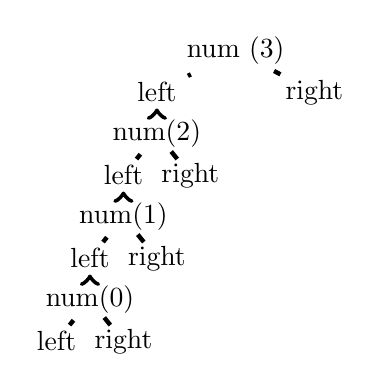
\begin{tikzpicture}
	[
	level distance=30pt,
	level 1/.style={sibling distance=4cm},
	level 2/.style={sibling distance=1.7cm},
	every node/.style = {
	},
	every child/.style = {
		ultra thick
	}
	]
{
\node{num (3)}
	child{node{left}
		child[->]{node{num(2)}
			child[-]{node{left}
				child[->]{node{num(1)}
					child[-]{node{left}
						child[->]{node{num(0)}
							child[-]{node{left}}
							child[-]{node{right}}}}
						child[-]{node{right}}}}
				child[-]{node{right}}
	}}
	child{node{right}};
}
\end{tikzpicture}
\end{center}
\end{figure}

Given this problems, a viable implementation of combinatorial games must look for alternative representations. Some possibilities are allowing surreal numbers to be represented with integers and floats or to store results of the tree traversals to minimize the number of times the complex tree structure must be analyzed. When looking at numbers strictly, the tree that resulted in a float or another chosen numerical representation may be discarded because it does not contain special information.

However, when changing the domain from surreal numbers to games, the tree cannot be always discarded. The reason for that is that the game tree may contain relevant information for gameplay. Although one could try keeping only the best move for each position in order to save space, the problem of adding games, that changes which move is best makes it difficult.

Consider the following draft:

\begin{lstlisting}
// CombinarotialGame.hpp
#include "everything_required.hpp"
using namespace std;

class CombinatorialGame {
  public:
	CombinatorialGame (vector<CombinatorialGame*> l,
					     vector<CombinatorialGame*> r);
	...
  private:
  	vector<CombinatorialGame*> left;
  	vector<CombinatorialGame*> right;
  	bool isSurreal;
  	bool isSwitch;
  	float realValue;
  	float bias;
  	float temperature;
};

\end{lstlisting}

\begin{lstlisting}
//CombinatorialGame.cpp
#include "path/to/CombinatorialGame.hpp"

CombinatorialGame::CombinatorialGame (
                    vector<CombinatorialGame*> l,
                    vector<CombinatorialGame*> r) {
	float maxL, minR;
	bool lFlag, rFlag;           
}
	
\end{lstlisting}

The draft handles some of the hard aspects of evaluation but a completed version contains solutions to many additional cases. The draft, for one, is incapable of handling infinite games, since there is no way interpretation for infinite structures. A more complete version can be found in CGSuite github repository, but the more important details are addressed.

\subsection*{Other Games To Play}

Now that vocabulary, methods and tools were introduced, this section brings some games to put your knowledge to proof.

\textbf{The Amazons} is a typical game that, like domineering, is fun and only requires pen and paper. Amazons is typically played in a 10x10 chess board with each player having four initial pieces in the fixed initial position depicted below. Each piece works just like a chess queen. In each turn, the player selects one of his/her queens and moves in an arbitrarily number of squares. Every square the amazon (queen) goes through is then burned from the game, making it so that no queen can move over it. The initial position in unimportant and the players can choose any starting position they find interesting.

\todo{image of typicall position}

For example, play may take place in an 8x8, a chessboard for convenience, with each player having two queen in opposing corners. Since, in this example, player Left is a beginner an Right is a seasoned player, Left has one additional queen next to one of his/her queens. It serves to show that there are no restrictions to the initial position - games do not have to be mathematically balanced to be fun.

\todo{image of given posi}

\textbf{The Angel Game} is more of a mathematical challenge more than a game, because it is not meant to actually be played. This game is played in a infinite squared board, with the Angel being located in of its cells. Each turn the Angel flies over $k$ squares and lands, depending on the desired rules. When it is the devils turn to play, it possesses a square from the infinite board. The challenge is to know whether, and for what values of $k$, the devil wins, given the Angel may not lend in a possessed square.

This game led to a lot of research until it was solved. Although it may not interest someone looking for a fun game it serves to show that even games on infinite boards are part of this theory. An important aspect of this game is that the position, after every move, becomes better and better for the devil, but still, sometimes it does not improve enough for the devil to win, even after an arbitrarily large number of moves.

\textbf{Snorts} is yet another fun game to be played with pen and paper. Snorts is a picture coloring game. Two herdsman, Bob that has a herd of bulls and Chad that had a herd of cows, compete to buy properties in a large open field. They are both interested in acquiring as many properties as possible, regardless of their sizes, but they respect each others space. Since cows cannot live next to bulls and vice-versa, Bob and Chad cannot buy any property next to each other.

The initial position for playing snorts is a partitioned shape. The initial position is somewhat problematic to draw, because may cause the first player to have easier tie playing. However, by making a large initial open space, it is harder to make a boring game. A good method to draw the board is to make a circle-like shape a start subdividing it randomly, making sure that there are not very large partitions. The picture below is an example of a snorts game in progress.

\todo{image}

\textbf{The Markswoman Amazons} is the first example of this section on how to create a game. This game is a variation of The Amazons, with one additional rule. After any movement is made, the Amazon that moved shoots an arrow in any direction that flies any number of squares, hitting and burning an open square. The arrow cannot hit other Amazons, but may target an already burned square. This serves to show how easy it is to adpat existing games.

\textbf{The Knights} is another possible variation of Amazons. The game has the same rules but uses chess knights instead of chess queens. This game may, for experienced chess players, seem less fun that the amazons, as it is much more predictable. It may be true, but, like the markswoman amazons may be worth trying.

...................














